\section{Introduction}]
The bulk of research into Compressive Sensing has been on designing efficient matrices to capture the signal, and on creating fast algorithms for the sample inversion. However, reconstructing a signal is not the only interesting signal processing task: there is also filtering, signal classification and inference based upon the signal. In this chapter, we investigate a method of applying ideas from Compressive Sensing to determine the occupancy of a spectral band, without ever reconstructing the singal from the samples as an intermediate step.

The purpose of the excercise is to drastically reduce the number of samples required to make a descsion about whether a band is occupied - for sensing matrices satisfying the RIP, the number of samples required to infer properties about the signal is considerably smaller than the number of samples required to reconstruct the signal. 

This chapter outlines the basic theory behind compressive inference, with some worked examples - estimating a single spike from compressed data, estimating a single rectangle from compressed data, and estimating synthetic frequency spectra from data. 

We begin by quickly review the RIP and its extension to stable embeddings, and how these ideas make it possible to infer properties about signals without reconstruction as intermediate step. We then define a maximum likelihood estimator to identify sparse components of a signal.

We then extend these ideas to the problem of maximum likelihood compressed estimation of a signal in some known set of basis functions. Finally, we apply these ideas to classification of a sequence of frequency bands. To our knowledge, this is the first time these techniques have been used to directly estimate spectral occupancy.

We demonstrate the efficiacy of our methods by computing ROC curves for noisy signals, at varying levels fo undersampling (from 5\% to 100\%) and at various levels of noise power.

\section{Theory}


The recent work of Candes and Tao \cite{Candes2006} and Donoho \cite{Donoho2006} has established that many real-world signals can be effectively captured via a small number of random projections relative to the dimension of the signal. For example, a 5 megapixel image can be thought of as a vector in \(\re^{5,000,000}\). However, it is well known that images have relatively few wavelet coefficients; this is exploited by the JPEG-2000 standard, which can represent the image as a 64-kb file (i.e a point in \(\re^{64,000}\).

Classically, for perfect signal reconstruction, we must sample a signal such that the sampling rate must be at least twice the maximum frequency in the bandlimited signal. The continuous time signal can then be recovered using an appropriate reconstruction filter (e.g. a sinc filter). For example, we can represent a sampled continuous signal as a multiplication of the signal with a train of Dirac delta functions at multiples of the sampling period T.
%
\begin{equation}
x\left(nT\right) = \Sh\left(t-nT\right)x\left(t\right)
\end{equation}
%
where
%
\begin{equation}
\Sh\left(t-nT\right) = \sum_{k=-\infty}^{\infty} \delta\left(t - kT\right)
\end{equation}

Working the frequency domain, this multiplication becomes convolution (which is equivalent to shifting):

\begin{equation}
\hat{X}_{s}\left(f\right) = \sum_{k=-\infty}^\infty x\left(t - kT\right)
\end{equation}

Thus if the spectrum of the frequency is supported on the interval \(\left(-B, B\right)\) then sampling at intervals \(\frac{1}{2B}\) will contain enough information to reconstruct the signal \(x(\left(t\right)\). Multiplying the spectrum by a rectangle function (low-pass filtering), to remove any images caused by the periodicity of the function, and the signal \(x(\left(t\right)\) can be reconstructed from its samples:

\begin{equation}
x\left(t\right) = \sum_{n=-\infty}^\infty x\left(nT\right) sinc\left(\frac{t_nT}{T}\right)
\end{equation}

In contrast Compressive Sampling suggests that by adding randomness into the measurement process, a sparse (or compressible signal) may be accurately sensed with far fewer measurements:
$y = Ax + w$

where \(A \in \mathbb{R}^{m \times n}\) is a matrix with random entries, \(x \in \mathbb{R}^n\) is the signal we capture, \(y \in \mathbb{R}^m\) is the result of the measurement process and \(w \sim N\left(0,1\right) \in \mathbb{R}^m\) is additive white Gaussian noise, \(m < n\).

Some technical conditions on the matrix \(A\) have to satisfied for it: namely the transformation defined by \(A\) must behave like an approximate Isometry, and it must be incoherent.

\begin{definition}[RIP]
We say that a matrix \(A\) satisifes the RIP of order \(\delta\) if \(\exists\) a \(\delta \in \left(0, 1\right)\) such that:
\begin{equation}
\left(1 - \delta\right) \vectornorm{x}_2^2 \leq \vectornorm{Ax}_2^2 \leq \left(1 + \delta\right) \vectornorm{x}_2^2
\end{equation}
i.e. \(A\) approximately preserves the lengths of all \(s\)-sparse vectors in \(\re^n\). 
\end{definition}

\begin{definition}[Coherence]
The mutual coherence of a matrix \(A\) is the absolute normalised inner product between different columns from \(A\). Denoting the \(k\)-th column in \(A\) by \(a_k\), the mutual coherence is given by:
\begin{equation}
\mu(A) = \max_{1\leq i,j\leq n , i\neq j} \frac{|\langle a^T_i, a_j\rangle|}{\vectornorm{a_i}_2\vectornorm{a_j}_2}
\end{equation}
\end{definition}

This implies that sensing with incoherent systems is good, and efficient mechanisms ought to acquire correlations with random waveforms (e.g. white noise).

\textbf{Theorem} \cite{Candes2006}
Fix x \(\in \mathbb{R}^n\) with a sparse coefficient basis, \(x_{i}\) in \(\psi\). Then a reconstruction from \(m\) random measurements is possible with probability \(1 - \delta\) if: 

\begin{equation}
m \geq C \mu^2(A) S \log\left(\frac{n}{\delta}\right)
\end{equation}
\label{minsamples}

where \( \mu(A)\) is the coherence of the two bases, and \(S\) is the number of non-zero entries on the support of the signal. 

In this new sensing paradigm, the complexity is shifted to the reconstruction process, where with high probability Donoho proved \cite{donoho2004neighborly}, that the minimiser of the program:

\begin{equation}
\argmin_{x} \frac{1}{2}\vectornorm{y-Ax}_2^2 + \lambda\vectornorm{x}_1
\end{equation}

coincides with the sparsest solution to the under-determined system of linear equations. Thus we are able to sense sparse signals with random waveforms, and reconstruct them via linear programming.

However, signal reconstruction is not the only interesting signal processing task. Filtering, classification, detection, and estimation are also required in real world systems. For these tasks it was thought that signal reconstruction must be performed first, and then classical signal processing techniques could be brought to bear on the reconstruction. 

There is some tension in this idea however: since the measurement matrix is an approximate isometry, some (as yet unspecified) operations on the measurements \(y\) should correspond to inference tasks (such as filtering and estimation) on \(x\). This means that performing inference needn’t require the reconstruction of the signal. 

The papers \cite{davenport2010signal} and \cite{davenport2007smashed} provide an introductory answer for the cases of filtering, detection, classification and estimation.

There has been a little work applying this line of work: \cite{schnelle2012compressive} shows how to design a Phase-Locked loop directly in the compressive domain and applies it to demodulating FM signals, and \cite{davenport2010wideband} extends this idea to a wideband compressive radio receiver. Matched filtering from compressive samples is performed in \cite{eftekhari2013matched}, and 

The structure of this document is as follows: sections \eqref{sec:prelims}, is a literature review of relevant material from compressed sensing, Wishart matrices, and maximum likelihood estimation of uncompressed signals in noise. Section \eqref{sec:estimation} gives an overview of the problem of estimating a signal from a known set of basis functions. 

\section{Compressive Estimation} \label{sec:estimation}
In this section, we develop some intuition into constructing estimators for the signal \(s\) directly on the compressive measurements:

\begin{equation}
y = As + n
\end{equation}
\\
where \(A \in \re^{m \times n} \), \(A_{ij} \sim \mathcal{N}\left(0,1/m\right)\), and \(n \in \re^n\) is AWGN. We again assume that \(s\) comes from a fixed set of models, parametrised by some set \(\Theta\). 

The likelihood for this model is, (as y is a normal random variable):

\begin{equation}
f\left(y \mid s\right) = \left(\frac{1}{\sqrt{2\pi}} \right)^m \exp{\left( - \frac{\left(y-As\right)^T  \left(y-As\right)}{2} \right)}
\end{equation}

Taking the logarithm and expanding, we find

\begin{equation}
\ln{f} = -y^Ty - s^TA^TAs + 2\langle y, As \rangle
\end{equation}

which is equal to:

\begin{equation}
ln{f} = - \vectornorm{y}_2^2 - \vectornorm{As}_2^2 + 2\langle y, As \rangle
\label{log-like}
\end{equation}
The first term of \eqref{log-like} is constant, for the same reasons as in section \eqref{sec:estimation}. The term 

\begin{equation}
\vectornorm{As}^2_2 = \langle As, As\rangle
\end{equation}

can be written as 

\begin{equation}
\langle A^T As, s\rangle
\end{equation}

We will replace this with its expectation \(\ep{\left( \langle A^T As, s\rangle \right)}\)

\begin{align*}
\ep{\left(\langle A^T As, s\rangle\right)} &=  \ep{\sum_{i=1}^n (A^TAs)^T_i s_i} \\
&= \sum_{i=1}^n \ep{(A^TAs)_i s_i} \\
&= \sum_{i=1}^n (\frac{1}{m}e_i s_i)^T_i s_i \\
&= \frac{1}{m} \langle s, s \rangle
\end{align*}

because

\begin{equation}
\ep{A^TA} = \frac{1}{m}I
\end{equation}

as it is a Wishart matrix (see section\ref{sec:prelims}). 
\\
So we can further approximate \eqref{log-like}:

\begin{equation}
\ln{f} = - \vectornorm{y}_2^2 + \frac{1}{m}\vectornorm{s}_2^2 + 2\langle y, As \rangle
\label{approx-log-like}
\end{equation}

The only, non-constant part of \eqref{approx-log-like} is the third term and so we define the estimator:

\begin{equation}
\hat{s} = \argmax_{\Theta} \langle y , As\left(\Theta\right)\rangle
\label{eq: compressive-estimator}
\end{equation}

For the case where \(s\) can be expanded in an orthonormal basis \(s = \sum_{i=1}^n \alpha_i\phi_i\), the maximum likelihood estimator is:

\begin{equation}
\hat{s} = \sum_{i=1}^n m\langle y, A\phi_i\rangle \phi_i
\end{equation}
\\
\\
Consider the case where \( y = As\) (no noise). Then

\begin{align*}
y^TA\phi_j &= \sum_i \alpha_i \phi_i^TA^TA\phi_j
\end{align*}

So 

\begin{align*}
y^TA\phi_j &= \sum_i \alpha_i \phi_i^TA^TA\phi_j \sim \frac{\alpha_i}{m} \delta_{ij}
\end{align*}

giving
 
\begin{equation}
\hat{\alpha_i} = m\left(y^TA\phi_j\right)
\end{equation}

\begin{remark}
The matrix \(M = A^TA\) is the projection onto the row-space of \(A\). It follows that \(\vectornorm{Ms}_2^2\) is simply the norm of the component of \(s\) which lies in the row-space of \(A\). This quantity is at most \(\vectornorm{s}_2^2\), but can also be \(0\) if \(s\) lies in the null space of \(A\). However, because \(A\) is random, we can expect that \(\vectornorm{Ms}_2^2\) will concentrate around \(\sqrt{m/n}\vectornorm{s}_2^2\) (this follows from the concentration property of sub-Gaussian random variables \eqref{cond:sub-Gauss concetration}).
\end{remark}

\subsection{Example: Single Spike}
We illustrate these ideas with a simple example: estimate which of \(n\) frequencies \(s\) is composed of.

A signal \(s \in \re^{300}\) composed of a single (random) delta function, with coefficients drawn from a Normal distribution (with mean 100, and variance 1) i.e 

\begin{equation}
s = \alpha_i \delta_i
\end{equation}
\\
with 

\begin{equation}
a_i \sim \mathcal{N}\left(100, 1\right)
\end{equation}

and the index \(i\) chosen uniformly at random from \([1, n]\).
\\
The signal was measured via a random Gaussian matrix \(A \in \re^{100 \times 300}\), with variance \(\sigma^2 = 1/
100 \) and the inner product between \(y = As\) and all 300 delta functions projected onto \(\re^{100}\) was calculated:

\begin{equation}
\hat{\alpha}_j = m\langle (A\alpha_i\delta_i), A\delta_j \rangle
\end{equation} 

We plot the \(\hat{\alpha_j}\) below, figure \ref{fig:new_basis_25}, (red circles), with the original signal (in blue, continuous line). Note how the maximum of the \(\hat{\alpha_j}\), coincides with the true signal.

\begin{figure}[h]
\centering
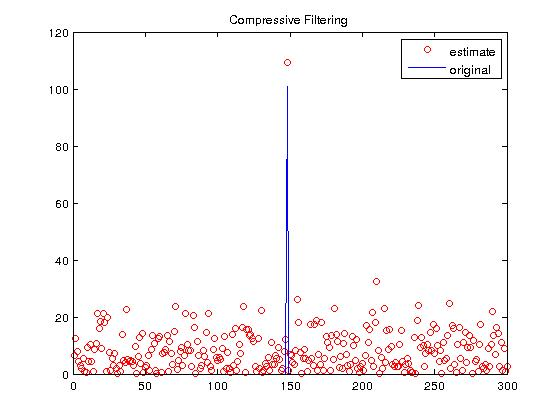
\includegraphics[height = 7.3 cm]{1spike_legend.jpg}
\caption{}
\label{fig:new_basis_25}
\end{figure}

\subsection{Estimating a single rectangle}

We show how to estimate the signal, composed of a single rectangle \eqref{fig:rectangle} expanded in the following basis

\begin{figure}[h]
\centering
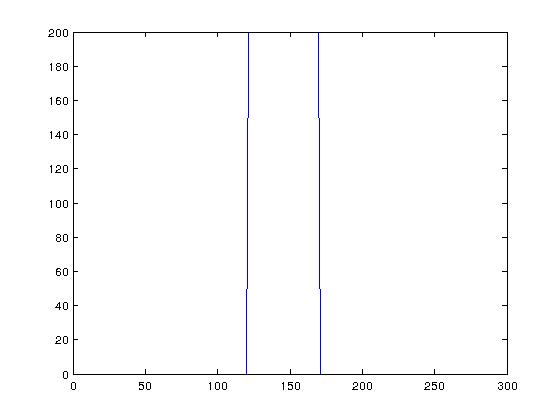
\includegraphics[height = 7.3 cm]{g.jpg}
\caption{}
\label{fig:rectangle}
\end{figure}

\begin{equation}
f_i\left(x\right) =
\begin{cases}
1 & \text{if } x \leq i \\
0 & \text{ otherwise } 
\end{cases}
\label{basis}
\end{equation}

We model our signal \(g\) as a linear combination of the basis functions (\ref{basis}):

\begin{equation}
g\left(x\right) = \sum_i a_i f_i 
\label{basis-expansion}
\end{equation}

To find the \(a_i\), we correlate (take the inner product of) the signal against the basis (\ref{basis}).

\begin{definition}
\begin{align}
h_j &= \langle g, f_j \rangle \\
&= \sum_j g\left(x\right) f_j\left(x\right) \\
&= \sum_j a_i f_i\left(x\right) f_j\left(x\right) \\
&= a_i \langle f_i, f_j\rangle \\
&\left(= \sum_{x=1}^j g\left(x\right)\right)
\end{align}
\end{definition}

As per the previous sections, we take compressive measurements:
\begin{equation}
y = Ag
\end{equation}
\\
where \(A \in \re^{m \times n} \), \(A_{ij} \sim \mathcal{N}\left(0,1/m\right)\), and then compute 
\begin{equation}
\langle y, Af_i\rangle = a_j  f_j^TA^tAf_j \sim \frac{a_j}{m} \langle f_j, f_i \rangle
\end{equation}
for the set of basis vectors \(f_1 \ldots f_n\) i.e. the estimator from the previous section, corresponding to this set of basis functions \eqref{eq: compressive-estimator}. 

We then form the vector 

\begin{equation}
\hat{h} = m \sum_i \langle y, Af_i\rangle f_j \sim h
\label{ss-estimator}
\end{equation}

An example can be seen in figure \ref{fig:hhat}, for a matrix \(A \in \re^{200 \times 300}.\)

\begin{figure}[h]
\centering
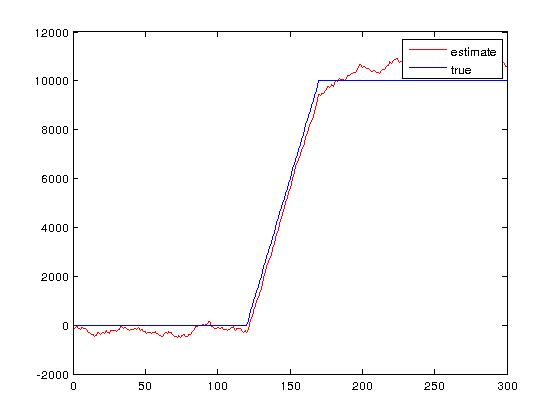
\includegraphics[height = 7.3 cm]{hhat.jpg}
\caption{}
\label{fig:hhat}
\end{figure}

\subsection{Estimating Frequency spectra}

Continuing from the previous (sub)-section we can create an estimate of \(g\), by the following procedure:

\begin{itemize}
\item Estimate the coefficients of the basis \(\hat{a}\) using \(\hat{a} = F^{-1} \hat{h}\)
\item Choose the \(k\) largest (for some \(k\) to be determined later).
\item Between the indices of the \(k\) \(\hat{a}\) take the average of the signal \(L^{-1}\hat{h}\).
\end{itemize}


\begin{figure}[h]
\centering
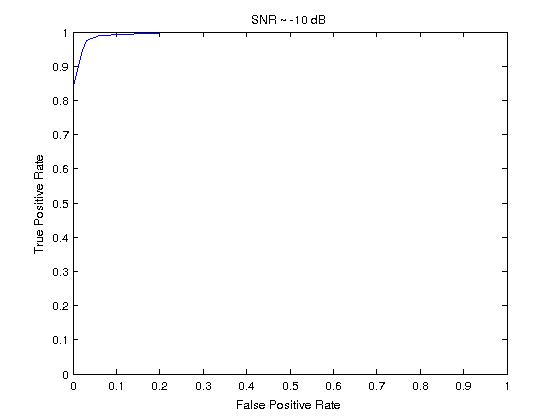
\includegraphics[height = 7.3 cm]{roc_minus_10.jpg}
\caption{ROC for synthetic data, midly noisy}
\label{fig:hvb}
\end{figure}

\begin{figure}[h]
\centering
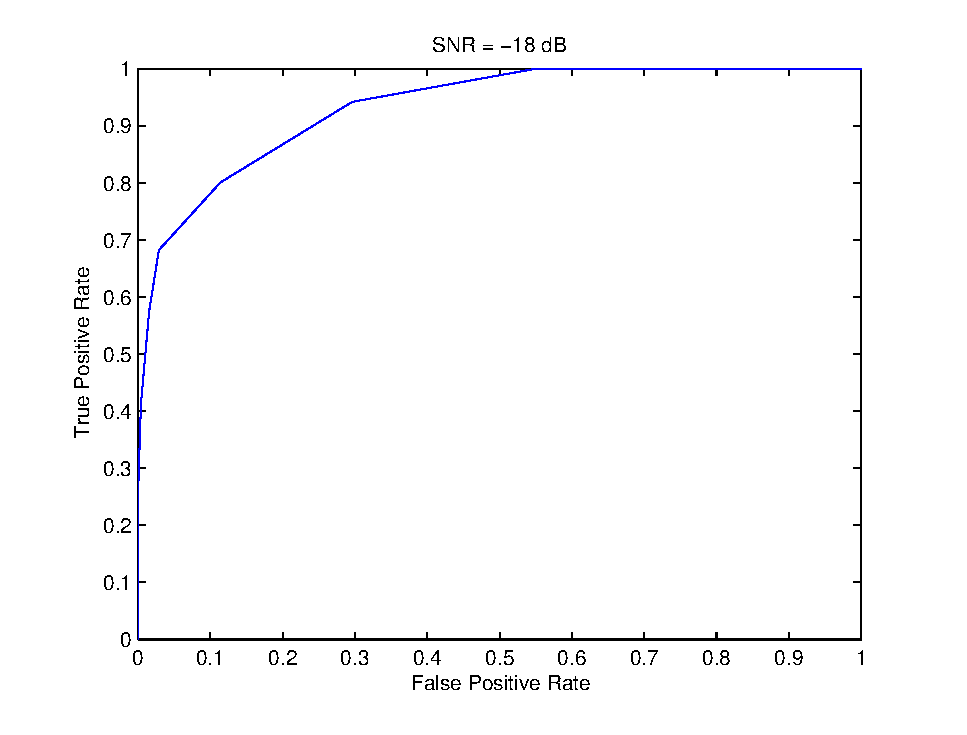
\includegraphics[height = 7.3 cm]{roc_minus_18.eps}
\caption{ROC for synthetic data, very noisy}
\label{fig:hvb}
\end{figure}